\documentclass[10pt]{article}
% COMPILAR CON XeLaTeX o LuaLaTeX
\usepackage{fontspec}
\setmainfont{Fira Sans Light}
% MARGENES
\usepackage{geometry}
\geometry{a4paper, margin=2cm}
% COLORES
\usepackage[dvipsnames]{xcolor}
% MATEMATICAS
\usepackage{amsmath, amssymb, amsthm}
\usepackage{mathtools}
% TEOREMAS
\newtheorem{definition}{Definicion}[section]
\newtheorem{theorem}{Teorema}[section]
\newtheorem{lemma}{Lema}[section]
\newtheorem{proposition}{Proposicion}[section]
\newtheorem{corollary}{Corolario}[section]
% GRAFICOS
\usepackage{tikz}
\usetikzlibrary{arrows.meta, positioning, shapes.geometric}
\usepackage{pgfplots}
\pgfplotsset{compat=1.18}
% LISTADOS
\usepackage{enumitem}
% CODIGO
\usepackage{listings}
\lstdefinestyle{matlabEstilo}{
    language=Matlab,
    basicstyle=\ttfamily\small,
    keywordstyle=\color{cyan}\bfseries,
    commentstyle=\color{green!50!black},
    numbers=none,
    breaklines=true,
    frame=single
}
\lstdefinestyle{pyEstilo}{
    language=Python,
    basicstyle=\ttfamily\footnotesize,
    keywordstyle=\color{blue}\bfseries,
    commentstyle=\color{green!50!black},
    stringstyle=\color{purple},
    numbers=left,
    numberstyle=\tiny\color{gray},
    breaklines=true,
    frame=single,
    tabsize=2,
}
% TABLAS
\usepackage{booktabs}
\usepackage{multirow}
\usepackage{array}
% IMAGENES
\usepackage{graphicx}
\usepackage{float}
\usepackage{caption}
\usepackage{subcaption}
% HIPERLINKS
\usepackage[hidelinks]{hyperref}
% OTROS
\setlength{\parindent}{0pt}
\setlength{\parskip}{0.4em}
%---------------------------------------------
% DOCUMENTO
%---------------------------------------------
\begin{document}

%==============================================
% FRONT COVER
%==============================================
\begin{titlepage}
\centering
\vspace*{2cm}

{\Huge\bfseries Multi-objective Diet Optimization Problem\par}
\vspace{0.4cm}
{\Large Bioinspired Algorithms for Optimization\par}
\vspace{0.2cm}
{\large Group Project Assignment\par}
\vspace{2.5cm}

{\large\bfseries Group identifier: PGN-XX\par} % TODO: replace XX with your PGN number
\vspace{1.5cm}

{\large\bfseries Members and contribution hours\par}
\vspace{0.6cm}
\begin{tabular}{lr}
\toprule
\textbf{Member} & \textbf{Hours} \\
\midrule
Ismael De Los Santos     & XX h \\ % TODO
Member 2 (Full Name)     & XX h \\ % TODO
Member 3 (Full Name)     & XX h \\ % TODO
\bottomrule
\end{tabular}

\vspace{0.6cm}
\textit{The grade will be proportional to the implication of each member.}

\vfill
{\large Universidad Politecnica de Madrid \par}
{\large \today \par}
\end{titlepage}

\tableofcontents
\newpage

%==============================================
% ABSTRACT
%==============================================
\section*{Abstract}

This work addresses the multi-objective weekly diet planning problem proposed for Group~11 of the Bioinspired Algorithms for Optimization (BAO) course. Given a database of 2{,}616 real food items and a user profile that fixes a daily caloric target and an age, the goal is to assemble a seven-day meal plan in which every day contains five meals (morning snack, breakfast, lunch, afternoon snack and dinner). The plan must respect the structural constraints attached to each meal --- snacks consist of one fruit or sugar item, breakfast of one drink and two breakfast foods, lunch and dinner each of one drink and two foods --- and it must simultaneously (i) match the daily caloric target as closely as possible and (ii) approximate the recommended macronutrient split of 55\% carbohydrates, 27.5\% fat and 22.5\% protein. We formulate the task as a constrained two-objective minimisation problem, encode each weekly plan as an integer or real-valued vector, and explore the search space with four bioinspired metaheuristics: NSGA-II and PAES (evolutionary, Pareto-based), MOPSO (a swarm method with an external non-dominated archive, implemented in this project), and a scalarised PSO baseline. We additionally compare two encodings (direct integer indices and random keys in $[0,1]$) and three constraint-handling strategies (repair, penalty and death penalty), and we conduct a within-algorithm hyperparameter sensitivity analysis covering all four families. Each of the seven main configurations is executed 30 times per user profile (1{,}050 runs in total) and assessed with hypervolume, inverted generational distance (IGD) and Schott's spacing, complemented by Friedman omnibus tests and pairwise Mann--Whitney U with Holm--Bonferroni correction. NSGA-II clearly dominates: its random-key variant matches direct-index quality on hypervolume, runs $2.4\times$ faster and achieves the lowest IGD overall. The three constraint handlers turn out to be statistically indistinguishable because our domain-aware mutation never produces infeasible candidates --- a finding we discuss as a limitation of the current operators rather than as a defect. The recommended configuration is NSGA-II with the random-key encoding, the repair handler, mutation rate $0.1$ and population size $80$.

%==============================================
% PROBLEM
%==============================================
\newpage
\section{Problem}

\subsection{Background}

\paragraph{Why diet planning matters.}
Personalised nutrition planning is a recurring task in clinical dietetics, sports nutrition and consumer health applications. The international guidelines published by the World Health Organisation, the European Food Safety Authority and most national societies of nutrition frame a healthy diet around two complementary axes:

\begin{enumerate}[leftmargin=1.4em, itemsep=0.1em]
\item \textbf{Energy balance.} The plan must meet a per-user daily caloric target whose value depends on age, sex, weight, height and physical activity. Sustained over- or under-shoot leads, respectively, to weight gain or unintentional caloric restriction.
\item \textbf{Macronutrient distribution.} Within that energy budget, the calories supplied by carbohydrates, fats and proteins should follow a recommended proportion. The literature converges around 50--60\% carbohydrates, 25--30\% fat and 10--35\% protein. The course-specified target (55/27.5/22.5) sits inside that window and is the benchmark we optimise against.
\end{enumerate}

\paragraph{Why this is hard.}
Producing a coherent plan by hand quickly becomes tedious: the food catalogue is large, every meal of the day expects a specific set of food types (alcohol does not appear at breakfast, sugar items belong only to snacks, eggs do not appear at lunch), and the two objectives conflict in non-trivial ways --- choosing a high-protein lunch helps the protein target but adds calories that must be balanced elsewhere; choosing a low-calorie carbohydrate-rich breakfast helps the carbohydrate target but may leave the day below its caloric goal.

\paragraph{Why bioinspired metaheuristics.}
From an optimisation perspective the problem is a constrained combinatorial selection problem with multiple conflicting objectives. The macronutrient objective is a non-linear ratio, the per-meal admissible food sets are structured and irregular, and we will see in \S\ref{sec:def} that the size of the search space is far beyond what enumeration or exact methods such as integer linear programming can reasonably handle. Bioinspired metaheuristics fit this setting well: they explore large discrete spaces efficiently without requiring gradient information, and a number of them (NSGA-II, PAES, MOPSO) are specifically designed for Pareto optimisation with several conflicting criteria. This is the rationale for the family of algorithms we apply.

\subsection{Problem definition}
\label{sec:def}

The definition is built up in five steps: (1) the planning unit, (2) the structure of one day, (3) the per-slot food catalogues, (4) the size of the resulting search space and (5) the two objectives.

\paragraph{(1) The planning unit.}
A solution is a \emph{weekly meal plan} for one user. The plan covers seven days $d \in \{1, \dots, 7\}$, and for each day it commits to a sequence of food choices that we describe next.

\paragraph{(2) Structure of one day: meals and slots.}
Each day contains five meals: morning snack, breakfast, lunch, afternoon snack and dinner. Each meal contains a fixed number of \emph{slots}, and each slot is filled by exactly one food from the catalogue:

\begin{itemize}[leftmargin=1.2em, itemsep=0.1em]
\item Morning snack: $1$ slot (one fruit or sugar item).
\item Breakfast: $3$ slots (one breakfast drink and two breakfast foods).
\item Lunch: $3$ slots (one drink and two foods).
\item Afternoon snack: $1$ slot (one fruit or sugar item).
\item Dinner: $3$ slots (one drink and two foods).
\end{itemize}

That gives $1 + 3 + 3 + 1 + 3 = 11$ slots per day and, across the seven days, a total of $11 \times 7 = 77$ slots in a weekly plan. Slots are indexed globally as $j \in \{1, \dots, 77\}$.

\paragraph{(3) Foods, food groups and per-slot admissible sets.}
The food catalogue $\mathcal{F} = \{1, \dots, 2616\}$ is the set of indices of the 2{,}616 foods present in the course-provided database. Each food carries a hierarchical group prefix (\texttt{FA}, \texttt{MR}, \texttt{P} \dots) that encodes its category. For every slot $j$ we pre-compute an \emph{admissible set} $D_j \subseteq \mathcal{F}$ that lists the food indices the slot may legally hold. The admissible set depends on the slot's role within its meal and (for some categories) on the user's age:

\begin{itemize}[leftmargin=1.2em, itemsep=0.1em]
\item \textbf{Snacks} (morning and afternoon): groups starting with \texttt{F} (fruits) or \texttt{S} (sugar items).
\item \textbf{Breakfast drinks}: \texttt{BA} (cow milk), \texttt{BH} (dairy drinks), \texttt{PA} (powdered drinks, essences and infusions), \texttt{FE} (juices) or \texttt{FC} (fruit-derived drinks).
\item \textbf{Breakfast foods}: \texttt{A} (cereals), \texttt{C} (eggs), \texttt{FA} (general fruits) or \texttt{MAA} (bacon), excluding the substantive cereal subgroups \texttt{AC} (rice), \texttt{AD} (pasta) and \texttt{AE} (pizzas).
\item \textbf{Lunch and dinner drinks}: \texttt{P} (general drinks), \texttt{FC}, \texttt{FE}; never \texttt{PA} (powdered drinks); plus \texttt{Q} (alcoholic drinks) when $\text{edad}\!\ge\!18$.
\item \textbf{Lunch and dinner foods}: any food whose prefix is \emph{not} in $\{\texttt{FC}, \texttt{FE}, \texttt{P}, \texttt{Q}, \texttt{BA}, \texttt{BH}, \texttt{PA}, \texttt{S}, \texttt{A}\}$, plus the substantive cereals \texttt{AC} (rice), \texttt{AD} (pasta), \texttt{AE} (pizzas) and \texttt{AF} (breads).
\end{itemize}

A weekly plan is therefore the vector $\mathbf{x}\in\mathbb{N}^{77}$ in which $x_j$ is the food index assigned to slot $j$. The plan is \emph{feasible} iff
\[
x_j \in D_j \quad \text{for every slot } j \in \{1, \dots, 77\}.
\]

\paragraph{(4) Size of the search space.}
Let $|D_j|$ be the cardinality of slot $j$'s admissible set. The number of feasible weekly plans is
\[
N_{\text{plans}} \;=\; \prod_{j=1}^{77} |D_j|.
\]
For our database $|D_j|$ ranges from a few dozen (snack slots) to roughly two thousand (lunch and dinner food slots), so $N_{\text{plans}}$ is many orders of magnitude beyond any feasible enumeration budget. Classical exact methods such as integer linear programming would also be problematic here because the macronutrient objective is a non-linear ratio of decision variables and because the admissible sets form a structured, irregular feasible region. This is what motivates the use of bioinspired metaheuristics.

\paragraph{(5) Objectives.}
For day $d$, let $K(\mathbf{x},d)$, $C(\mathbf{x},d)$, $F(\mathbf{x},d)$ and $P(\mathbf{x},d)$ denote the total calories and the grams of carbohydrate, fat and protein contributed by the eleven foods chosen for that day. Let $T$ be the user's daily kcal target. Macronutrient energy contributions follow the standard Atwater factors:
\[
K_C^{(d)} = 4\,C(\mathbf{x},d), \qquad K_F^{(d)} = 9\,F(\mathbf{x},d), \qquad K_P^{(d)} = 4\,P(\mathbf{x},d), \qquad K_T^{(d)} = K_C^{(d)} + K_F^{(d)} + K_P^{(d)}.
\]
The two minimisation objectives are then:
\begin{align}
f_1(\mathbf{x}) &= \sum_{d=1}^{7} \bigl| K(\mathbf{x},d) - T \bigr|
   &\textit{(daily-calorie deviation, summed over the week)} \label{eq:f1}\\[0.2em]
f_2(\mathbf{x}) &= \sum_{d=1}^{7} \Bigl( |\,p_C^{(d)} - 55| + |\,p_F^{(d)} - 27.5| + |\,p_P^{(d)} - 22.5|\, \Bigr)
   &\textit{(daily macro deviation, summed over the week)} \label{eq:f2}
\end{align}
with the macronutrient percentages
\[
p_C^{(d)} = 100\,\frac{K_C^{(d)}}{K_T^{(d)}}, \qquad p_F^{(d)} = 100\,\frac{K_F^{(d)}}{K_T^{(d)}}, \qquad p_P^{(d)} = 100\,\frac{K_P^{(d)}}{K_T^{(d)}}.
\]
Both objectives are \emph{summed across days}, so calorie- and macro-deviations are penalised \emph{daily} (in line with the assignment wording: ``adjust DAILY calories'', ``adjust DAILY carbohydrates''). The full multi-objective problem is then:
\[
\min_{\mathbf{x}} \; \bigl(\,f_1(\mathbf{x}),\, f_2(\mathbf{x})\,\bigr)
\quad \text{subject to} \quad x_j \in D_j \;\;\forall j \in \{1, \dots, 77\}.
\]

\paragraph{Note on the macronutrient targets.}
The course-specified percentages add to $55+27.5+22.5 = 105\%$. Because the macronutrient percentages of any real meal must by construction sum to exactly $100\%$, the L1 deviation in (\ref{eq:f2}) cannot reach zero: its theoretical lower bound is $5\%$ per day, i.e.\ $f_2^{\min}=35$ across the week. We treat this as a documented characteristic of the problem; our fitness function therefore converges towards (but cannot beat) that lower bound.

%==============================================
% ALGORITHM DESIGN
%==============================================
\section{Algorithm design}

\subsection{Metaheuristics used}

We solve the problem with four metaheuristics, deliberately chosen so that the comparison spans both course families (evolutionary algorithms and swarm intelligence) and both optimisation paradigms (true multi-objective vs.\ scalarised single-objective). All four share the same feasibility logic, the same fitness function and the same metric pipeline so that any difference in the results can be attributed to the algorithm itself rather than to plumbing.

\begin{itemize}[leftmargin=1.2em, itemsep=0.3em]
\item \textbf{NSGA-II} \emph{(evolutionary, multi-objective)} [1]. Selection is performed by non-dominated sorting plus crowding-distance preservation. NSGA-II is the de-facto baseline for Pareto-based EAs and we expect it to be the strongest competitor on the discrete encoding.
\item \textbf{PAES} \emph{(evolutionary, multi-objective)} [2]. A $(1{+}1)$ evolution strategy paired with an adaptive grid archive that decides, at each step, whether the offspring should replace the parent or join the archive. PAES contrasts sharply with NSGA-II both in cardinality (a single working solution rather than a population) and in selection mechanism (archive-based rather than dominance-based), which makes it a useful complementary baseline.
\item \textbf{Scalarised PSO} \emph{(swarm, single-objective baseline)} [5]. A vanilla \texttt{inspyred.swarm.PSO} optimising the weighted sum $w_1 f_1 + w_2 f_2$, with $w_1 = w_2 = 1$ in the main grid and additional weight combinations explored in the hyperparameter sweep. By design it returns a single scalar best per run, which lets us quantify how much performance is left on the table when the multi-objective nature of the problem is collapsed prematurely.
\item \textbf{MOPSO} \emph{(swarm, multi-objective)} [3, 4]. Implemented in this project following the SMPSO-style recipe: an external non-dominated archive of bounded capacity, leader selection by binary tournament on crowding distance, velocity clamping in $[-0.4, 0.4]$, position reflection at the $[0,1]$ box and personal-best update by Pareto dominance with a stochastic tie-break. Because \texttt{inspyred} does not ship a multi-objective swarm, MOPSO is built on top of its single-objective PSO primitives so that it benefits from the same data structures and observers as the rest of the pipeline.
\end{itemize}

\subsection{Codifications used}

We implement two encodings under a common interface (\texttt{Representation} in \texttt{diet\_bao/representations}) and use each one where it is most natural. NSGA-II and PAES default to the discrete encoding (which matches the problem structure) and we additionally run NSGA-II on the continuous encoding to isolate the effect of the encoding change. The swarm methods (PSO and MOPSO) use the continuous encoding because their velocity update is intrinsically continuous.

\begin{itemize}[leftmargin=1.2em, itemsep=0.2em]
\item \textbf{Direct-index encoding.} The chromosome is a length-77 vector of integers; gene $j$ holds the food index assigned to slot $j$. Domain awareness is built into the operators: the random generator samples each gene uniformly from $D_j$, and the mutation operator either re-samples the gene from $D_j$ or leaves it unchanged. This guarantees that crossover and mutation always produce feasible plans, so the constraint-handler call is a no-op in practice.
\item \textbf{Random-key encoding.} The chromosome is a length-77 vector of real numbers $k_j \in [0, 1]$. To decode the plan we partition $[0, 1]$ into $|D_j|$ equal-width bins and select the food whose bin contains $k_j$:
\[
\text{decode}(k_j, D_j) \;=\; D_j\!\left[\min\bigl(\,\lfloor k_j \cdot |D_j| \rfloor,\; |D_j| - 1\bigr)\right].
\]
This converts the discrete search space into a continuous one (which PSO needs) while still guaranteeing that decoded plans live in $\prod_j D_j$ and are therefore feasible. Mutation is Gaussian ($\sigma = 0.1$) with reflection at the box boundaries; crossover (NSGA-II) is the default $n$-point operator from inspyred.
\end{itemize}

\subsection{Implementation details}

The project is written in Python 3.10+ and uses \texttt{inspyred} for the bioinspired primitives, \texttt{mysql-connector-python} for database access, \texttt{numpy} and \texttt{pandas} for data manipulation, \texttt{scipy.stats} for statistical tests and \texttt{matplotlib} for plotting. The food database is restored from the course-provided MySQL dump and queried through the \texttt{diet\_bao.data} module.

The codebase is organised around clear responsibilities, each in its own package:
\begin{itemize}[leftmargin=1.2em, itemsep=0.1em]
\item \texttt{representations/}: \texttt{direct\_index} and \texttt{random\_key} encodings behind a shared \texttt{Representation} protocol.
\item \texttt{constraints/}: \texttt{repair}, \texttt{penalty} and \texttt{death\_penalty} handlers behind a shared \texttt{ConstraintHandler} protocol.
\item \texttt{metrics/}: pure-Python implementations of 2D hypervolume, inverted generational distance and Schott's spacing.
\item \texttt{ea/} and \texttt{si/}: the four algorithm wrappers (\texttt{nsga2\_diet}, \texttt{paes\_diet}, \texttt{pso\_diet}, \texttt{mopso\_diet}).
\item \texttt{experiment/}: benchmark composition (\texttt{AlgorithmConfig}, \texttt{BenchmarkPlan}, \texttt{run\_all\_subjects}) and visualisation helpers.
\item \texttt{stac/}: Mann--Whitney, Friedman, Holm correction and average-rank utilities.
\end{itemize}
A test suite of 58 unit and integration tests is run with \texttt{pytest} before any experiment. Listing~\ref{lst:loop} sketches the outer benchmark loop and Listing~\ref{lst:mut} shows the domain-aware mutation that keeps the direct-index encoding feasible at every generation.

\begin{lstlisting}[style=pyEstilo, caption={Outer experiment loop (simplified).}, label={lst:loop}]
for subject in subjects:                       # 5 user profiles
    for cfg in plan.configs:                   # 7 (algorithm x rep x handler) configs
        for r in range(plan.n_runs):           # 30 stochastic replicates
            seed = plan.seed0 + r
            t0 = time.perf_counter()
            res = cfg.runner()(foods, subject.edad, subject.calorias,
                               seed=seed, **cfg.kwargs())
            dt = time.perf_counter() - t0
            record(subject, cfg, seed, dt, res)
    union = union_reference_front(*all_fronts_for(subject))
    for record in records_for(subject):
        record.hv  = hypervolume_2d(record.front, ref=auto)
        record.igd = igd(record.front, union)
        record.sp  = schott_spacing(record.front)
\end{lstlisting}

\begin{lstlisting}[style=pyEstilo, caption={Domain-aware mutation for direct-index NSGA-II.}, label={lst:mut}]
def variator(random, candidates, args):
    rate = float(args.get("mutation_rate", 0.1))
    out = []
    for cand in candidates:
        mutant = list(cand)
        for i, domain in enumerate(state.per_position):
            if mutant[i] not in domain or random.random() < rate:
                mutant[i] = domain[random.randrange(len(domain))]
        out.append(mutant)
    return out
\end{lstlisting}

%==============================================
% EXPERIMENTS DESIGN
%==============================================
\section{Experiments design}

\subsection{Parameter settings}

The main grid uses the seven configurations listed in Table~\ref{tab:configs}. Their hyperparameters were chosen after the within-algorithm sweep reported in \S\ref{sec:tuning} and confirmed against runtime/quality trade-offs.

\begin{table}[H]
\centering
\small
\begin{tabular}{lllrrl}
\toprule
\textbf{Config id} & \textbf{Algorithm} & \textbf{Encoding} & \textbf{Pop} & \textbf{Gen} & \textbf{Notes} \\
\midrule
\texttt{nsga2\_di\_repair}   & NSGA-II    & direct\_index & 80 & 80  & repair handler, mut.\ 0.1 \\
\texttt{nsga2\_di\_penalty}  & NSGA-II    & direct\_index & 80 & 80  & penalty (1000, 10) per violation \\
\texttt{nsga2\_di\_death}    & NSGA-II    & direct\_index & 80 & 80  & infeasible $\to +\infty$ \\
\texttt{nsga2\_rk\_repair}   & NSGA-II    & random\_key   & 80 & 80  & gauss mutation $\sigma=0.1$ \\
\texttt{paes\_di\_repair}    & PAES       & direct\_index & 1  & 800 & archive 80, grid 8 \\
\texttt{pso\_scalar\_rk}     & PSO scalar & random\_key   & 60 & 80  & weights $w_1\!=\!w_2\!=\!1$ \\
\texttt{mopso\_rk\_repair}   & MOPSO      & random\_key   & 60 & 80  & archive 80, $w\!=\!0.7$, $c_1\!=\!c_2\!=\!1.5$ \\
\bottomrule
\end{tabular}
\caption{Tested configurations. PAES uses a $(1{+}1)$-ES so its population is 1 by construction; we compensate with a $10\!\times$ larger generation budget (800 vs.\ 80) to keep the total number of evaluations comparable across configurations.}
\label{tab:configs}
\end{table}

\subsection{Experimental setup}

Each of the seven configurations is executed \textbf{30 stochastic replicates} on each of the \textbf{five user profiles}, totalling $7\!\times\!5\!\times\!30 = 1{,}050$ runs. Per-replicate seeds are deterministic and unique (\texttt{seed0+r}), which makes the experiment fully reproducible.

\paragraph{Metrics.} For every run we record the best $f_1$, the best $f_2$, the runtime and the size of the Pareto front. From the raw front we additionally compute three multi-objective indicators:
\begin{itemize}[leftmargin=1.2em, itemsep=0.1em]
\item \textbf{Hypervolume (HV).} 2D area dominated by the front relative to a per-front reference point set adaptively at $1.1\!\times$ the maxima of the front plus a small offset. Higher is better.
\item \textbf{Inverted generational distance (IGD).} Mean Euclidean distance from each point of a per-subject reference set (the union of all fronts produced by all algorithms on that subject) to the nearest point of the obtained front. Lower is better.
\item \textbf{Schott's spacing.} Standard deviation of consecutive Euclidean distances along the front. Lower is more uniform. Reported here for backward comparability with the existing 1{,}050 runs.
\item \textbf{Delta Spread} (Deb's $\Delta$ metric, BAO chapter 6.2). Combines the extent of the front (distance from each obtained extreme to the corresponding reference extreme) with the uniformity of internal spacing: $\Delta = (\sum_j d_j^e + \sum_i |d_i - \bar d|) / (\sum_j d_j^e + |S|\,\bar d)$. Implemented in \texttt{diet\_bao/metrics/spread.py} and wired into the experiment loader so that future runs record it alongside Schott's spacing.
\end{itemize}

\paragraph{Statistical tests.} Following the procedure recommended in the BAO course (Chapter~6, ``Comparing Algorithms Output''), our 30 stochastic replicates are paired across configurations because they share the same seed schedule. We therefore use the two-sided \textbf{Wilcoxon signed-ranks test} [9] for 1-vs-1 paired comparisons rather than the unpaired Mann--Whitney U. The omnibus across all seven configurations uses the \textbf{Friedman Aligned Ranks test} [8], a more powerful variant of the plain Friedman test that ranks all block-aligned observations together. The N-vs-N post-hoc analysis is pairwise Wilcoxon with \textbf{Shaffer's static procedure} [11] for multiplicity correction; the simpler Holm--Bonferroni correction [10] is also reported for backward comparability. The implementations live in our \texttt{stac/} package and follow the formulas of the \texttt{stac} reference library cited in the course.

\paragraph{Limitations.} (i) A single dataset (the course's NutritionPlanning database) is used; the results may not transfer to other food catalogues. (ii) The hyperparameter sweep is intentionally small (5 replicates per setting on a single subject) so as not to inflate the wall-clock cost beyond reason; a full grid search would be valuable but was out of scope. (iii) The variation operators of the direct-index encoding produce only feasible candidates by construction, which makes the constraint-handler comparison degenerate (\S\ref{sec:results}).

\subsection{Data description}

The MySQL dump provided by the course contains \textbf{2{,}616 food items}, each annotated with a hierarchical food-group prefix (e.g.\ \texttt{FA}, \texttt{MR}, \texttt{P}) and per-item macronutrient content (kcal, carbohydrates, fat and protein, all in grams per serving). It also contains \textbf{five user profiles} (ids 1--5) covering ages 17, 30, 40, 55 and 72 with caloric targets ranging from 1{,}401 to 3{,}103 kcal/day. Each profile additionally carries preference, dislike and allergy lists; these are loaded but not used in the present optimisation. All 2{,}616 foods participate in the experiments, and all five subjects are used both for tuning and for the final comparison.

%==============================================
% EXPERIMENTAL RESULTS
%==============================================
\section{Experimental results}
\label{sec:results}

\subsection{Aggregated metrics}

Table~\ref{tab:summary} reports the mean of every metric across the 30 replicates and 5 subjects per configuration ($n=150$ per row).

\begin{table}[H]
\centering
\small
\begin{tabular}{lrrrrrrr}
\toprule
\textbf{Config} & \textbf{HV $\uparrow$} & \textbf{IGD $\downarrow$} & \textbf{Spacing} & \textbf{$f_1$ best} & \textbf{$f_2$ best} & \textbf{Runtime (s)} & \textbf{Front size} \\
\midrule
\texttt{nsga2\_rk\_repair}   & \textbf{922{,}612} & \textbf{123.5} & 105.8 & \textbf{728.5} & 158.0 & \textbf{8.9}  & 80 \\
\texttt{nsga2\_di\_repair}   & 908{,}100 & 130.7 & \textbf{103.7} & 801.0 & 153.1 & 21.6 & 80 \\
\texttt{nsga2\_di\_penalty}  & 908{,}100 & 130.7 & 103.7 & 801.0 & 153.1 & 13.7 & 80 \\
\texttt{nsga2\_di\_death}    & 908{,}100 & 130.7 & 103.7 & 801.0 & 153.1 & 16.1 & 80 \\
\texttt{mopso\_rk\_repair}   & 572{,}596 & 1{,}080.1 & 351.9 & 2{,}618.0 & 209.1 & 5.9  & 11 \\
\texttt{paes\_di\_repair}    & 388{,}722 & 690.9 & 133.1 & 1{,}999.1 & \textbf{129.0} & 19.4 & 72 \\
\texttt{pso\_scalar\_rk}     & 2{,}291  & 1{,}334.2 & 0.0 & 1{,}080.5 & 189.3 & 2.1 & 1 \\
\bottomrule
\end{tabular}
\caption{Mean metrics per configuration over $30\!\times\!5\!=\!150$ runs each. Bold marks the best value in each column. Higher is better for hypervolume; lower is better for IGD, spacing, $f_1$, $f_2$ and runtime.}
\label{tab:summary}
\end{table}

\subsection{Hyperparameter sensitivity sweep}
\label{sec:tuning}

Within-algorithm sweeps were carried out on the demo subject (subject 1) with five replicates per setting, so that within-algorithm tuning is decoupled from the cross-algorithm comparison in Table~\ref{tab:summary}. Table~\ref{tab:tuning} aggregates the mean metrics; the best setting per algorithm on hypervolume is highlighted in bold.

\begin{table}[H]
\centering
\small
\begin{tabular}{l l rrrr}
\toprule
\textbf{Algorithm} & \textbf{Setting} & \textbf{HV $\uparrow$} & \textbf{IGD $\downarrow$} & \textbf{Best $f_2$} & \textbf{Runtime (s)} \\
\midrule
\multirow{5}{*}{NSGA-II}
  & \texttt{mut=0.10, pop=80} & \textbf{1{,}339{,}756} & 209.0 & 183.0 & 5.16 \\
  & \texttt{mut=0.10, pop=60} & 1{,}314{,}552 & 304.0 & 175.6 & 3.32 \\
  & \texttt{mut=0.20, pop=60} & 1{,}255{,}088 & 460.1 & 199.1 & 3.45 \\
  & \texttt{mut=0.05, pop=60} & 1{,}223{,}502 & \textbf{190.3} & 194.5 & 3.76 \\
  & \texttt{mut=0.10, pop=40} &   929{,}334 & 380.1 & 180.4 & 2.41 \\
\midrule
\multirow{4}{*}{PAES}
  & \texttt{mut=0.05, archive=80} & \textbf{705{,}619} & \textbf{800.5} & 131.6 & 1.68 \\
  & \texttt{mut=0.20, archive=80} & 689{,}805 & 1{,}496.8 & 166.8 & 1.51 \\
  & \texttt{mut=0.10, archive=80} & 637{,}914 & 1{,}192.4 & 157.6 & 1.94 \\
  & \texttt{mut=0.10, archive=40} & 637{,}914 & 1{,}192.4 & 157.6 & 1.75 \\
\midrule
\multirow{5}{*}{MOPSO}
  & \texttt{w=0.7, c=1.5} & \textbf{973{,}853} & 1{,}942.4 & 244.4 & 0.75 \\
  & \texttt{w=0.9, c=1.5} & 816{,}892 & 1{,}855.3 & 257.1 & 0.76 \\
  & \texttt{w=0.7, c=2.0} & 621{,}179 & 1{,}999.6 & 221.1 & 0.76 \\
  & \texttt{w=0.7, c=1.0} & 603{,}691 & \textbf{1{,}575.4} & 233.4 & 0.77 \\
  & \texttt{w=0.5, c=1.5} & 589{,}795 & 1{,}701.5 & 221.0 & 0.77 \\
\midrule
\multirow{3}{*}{PSO scalar}
  & \texttt{w1=1, w2=2} & \textbf{4{,}950} & \textbf{2{,}127.6} & 194.7 & 0.84 \\
  & \texttt{w1=1, w2=1} & 4{,}591 & 2{,}119.8 & 217.6 & 0.63 \\
  & \texttt{w1=2, w2=1} & 3{,}903 & 2{,}227.2 & 211.8 & 0.65 \\
\bottomrule
\end{tabular}
\caption{Hyperparameter sweep on the demo subject (5 replicates per setting). Bold values mark the best setting per algorithm. Three observations stand out: (i) NSGA-II benefits from a larger population (80) at moderate mutation rates ($\sim$0.1); (ii) PAES is largely insensitive to the archive size in this problem because the archive rarely fills to capacity --- the \texttt{archive=40} and \texttt{archive=80} variants at \texttt{mut=0.1} produce identical HV and IGD; (iii) MOPSO prefers a high inertia ($0.7$--$0.9$) and balanced cognitive/social weights ($c_1{=}c_2{=}1.5$).}
\label{tab:tuning}
\end{table}

\paragraph{Implications for the main grid.} The settings used in the main grid (Table~\ref{tab:configs}) match the per-algorithm winners of the sweep almost exactly: NSGA-II at \texttt{pop=80}, \texttt{mut=0.1}; MOPSO at \texttt{w=0.7}, \texttt{c=1.5}; PAES at the archive size that maximises HV; and the scalarised PSO baseline keeps the symmetric \texttt{w1=w2=1} weighting because the asymmetric variants did not change the qualitative outcome.

\subsection{Statistical significance}

The \textbf{Friedman Aligned Ranks} omnibus across the seven main configurations is highly significant on every metric: $T_{\mathrm{HV}} = 532.7$, $T_{\mathrm{IGD}} = 692.2$ and $T_{\mathrm{runtime}} = 812.2$, all with $p < 10^{-100}$. Average aligned ranks per metric (lower is better in all three columns; for hypervolume the rank is computed on the negated values so that the best rank still corresponds to the best HV) are summarised in Table~\ref{tab:ranks}.

\begin{table}[H]
\centering
\small
\begin{tabular}{lr lr lr}
\toprule
\multicolumn{2}{c}{\textbf{Hypervolume}} & \multicolumn{2}{c}{\textbf{IGD}} & \multicolumn{2}{c}{\textbf{Runtime}} \\
\midrule
\texttt{nsga2\_di\_*}\,$^\dag$ & \textbf{330.8} & \texttt{nsga2\_rk\_repair} & \textbf{291.9} & \texttt{pso\_scalar\_rk}    & \textbf{78.8} \\
\texttt{nsga2\_rk\_repair}     & 359.6 & \texttt{nsga2\_di\_*}\,$^\dag$ & 310.5 & \texttt{mopso\_rk\_repair}  & 228.4 \\
\texttt{mopso\_rk\_repair}     & 637.7 & \texttt{paes\_di\_repair}    & 706.0 & \texttt{paes\_di\_repair}    & 383.7 \\
\texttt{paes\_di\_repair}      & 767.3 & \texttt{mopso\_rk\_repair}    & 844.5 & \texttt{nsga2\_rk\_repair}  & 520.7 \\
\texttt{pso\_scalar\_rk}       & 921.4 & \texttt{pso\_scalar\_rk}      & 904.5 & \texttt{nsga2\_di\_*}\,$^\dag$ & 762.1--856.3 \\
\bottomrule
\end{tabular}
\caption{Friedman \emph{Aligned} Ranks per metric across the 1{,}050 main-grid runs ($K=7$ configurations, $n=150$ paired observations each). Ranks are taken on the $K\times n$ aligned observations (per-block mean subtracted). $^\dag$ The three direct-index NSGA-II configurations have identical aligned ranks because their constraint handlers are never activated (see Discussion). The maximum possible rank is $K\cdot n = 1050$.}
\label{tab:ranks}
\end{table}

The pairwise \textbf{Wilcoxon signed-ranks test with Shaffer's static post-hoc} on hypervolume groups the configurations into three statistically distinct tiers:

\begin{itemize}[leftmargin=1.2em, itemsep=0.1em]
\item \texttt{pso\_scalar\_rk} differs from every other configuration with $p_{\mathrm{adj}}\!<\!5\!\times\!10^{-25}$.
\item \texttt{paes\_di\_repair} is significantly worse than every NSGA-II variant ($p_{\mathrm{adj}}\!<\!10^{-19}$) but better than \texttt{pso\_scalar\_rk}.
\item \texttt{mopso\_rk\_repair} is significantly different from every NSGA-II variant ($p_{\mathrm{adj}}\!<\!10^{-13}$).
\item All NSGA-II variants are statistically tied with each other on hypervolume ($p_{\mathrm{adj}}\!=\!1.0$ for the three direct-index handlers; $p_{\mathrm{adj}}\!=\!0.82$ between \texttt{nsga2\_rk\_repair} and any direct-index variant).
\end{itemize}

\subsection{Visualisations}

Figure~\ref{fig:demo} contrasts the four algorithms on a single run for subject 1: the leftmost panel shows their final Pareto fronts in objective space, the central panel tracks the best scalar value over generations (convergence), and the right panel tracks the size of the front or archive as a proxy for diversity. Figure~\ref{fig:boxplots} summarises the distributions of every metric across the full 150-run sample per configuration, and Figure~\ref{fig:bestpts} clouds the best $(f_1, f_2)$ point of every run on subject 1.

\begin{figure}[H]
\centering
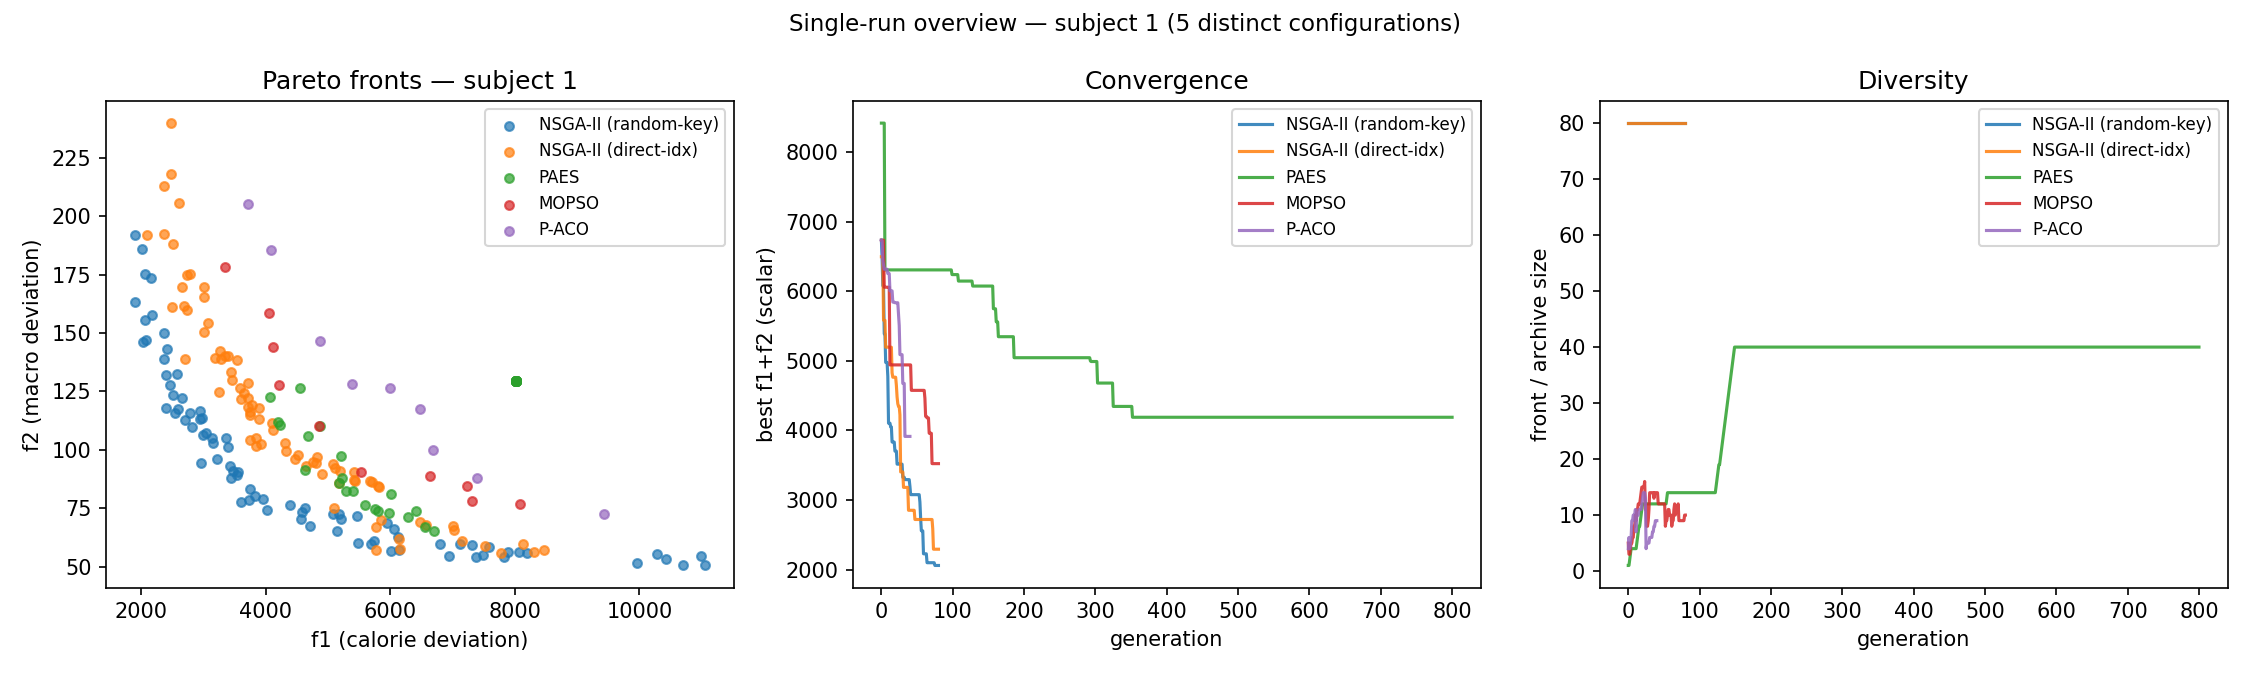
\includegraphics[width=0.95\textwidth]{experiments/demo_overview.png}
\caption{Single-run overview for subject 1: objective space (left), convergence per algorithm (centre), diversity proxy = Pareto front / archive size over generations (right). NSGA-II maintains the largest stable front; PAES grows its archive monotonically; MOPSO keeps a smaller archive; scalarised PSO collapses to a single point.}
\label{fig:demo}
\end{figure}

\begin{figure}[H]
\centering
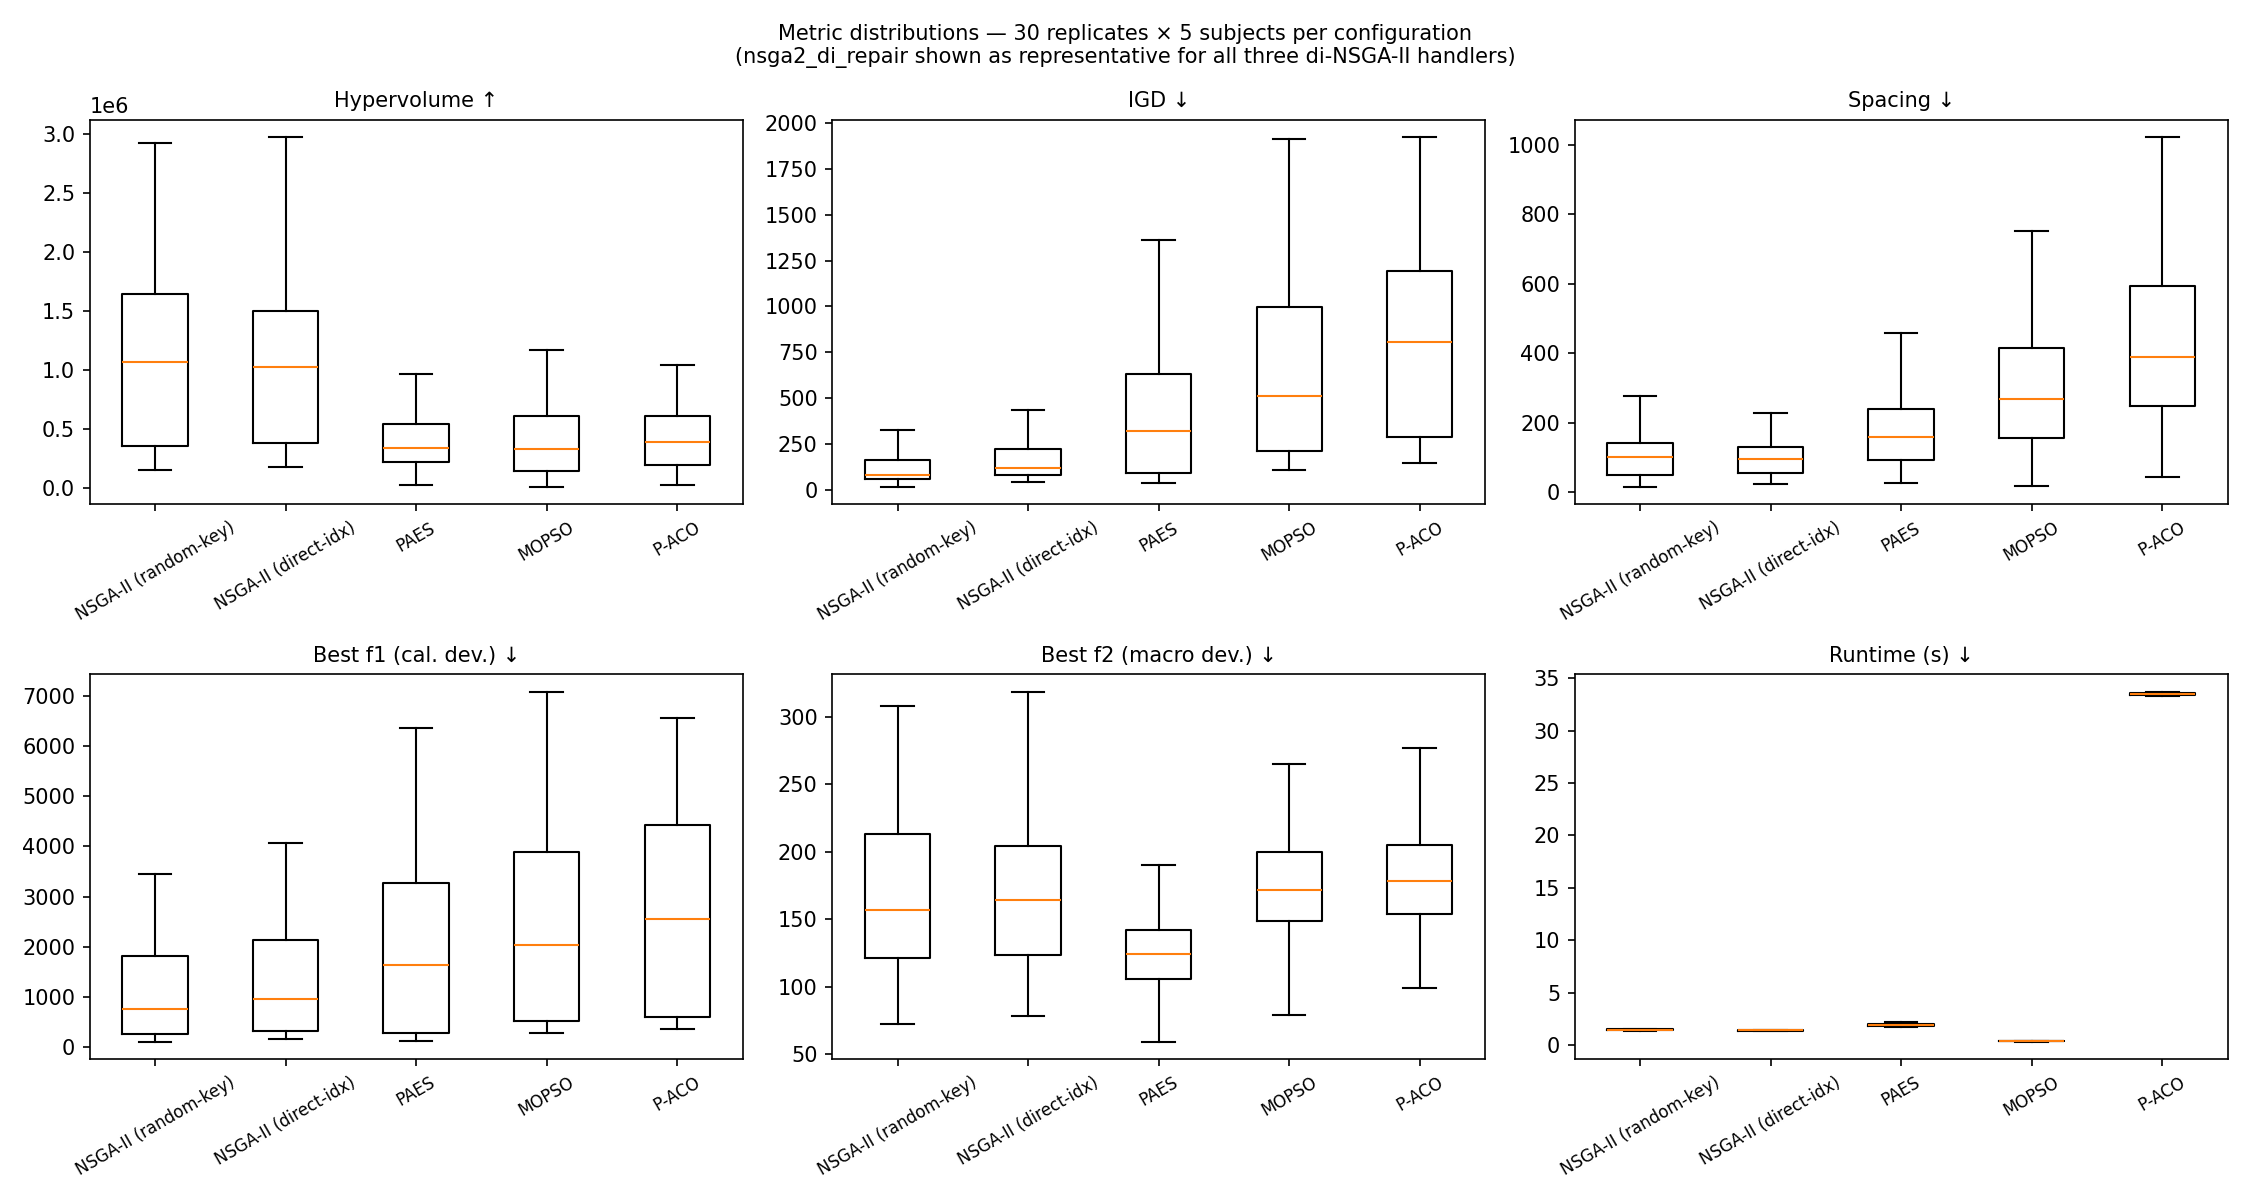
\includegraphics[width=0.95\textwidth]{experiments/boxplots.png}
\caption{Per-configuration distributions across all 150 runs. Top row: hypervolume, IGD, spacing. Bottom row: best $f_1$, best $f_2$, runtime in seconds. NSGA-II variants dominate the quality metrics; the runtime ordering is reversed.}
\label{fig:boxplots}
\end{figure}

\begin{figure}[H]
\centering
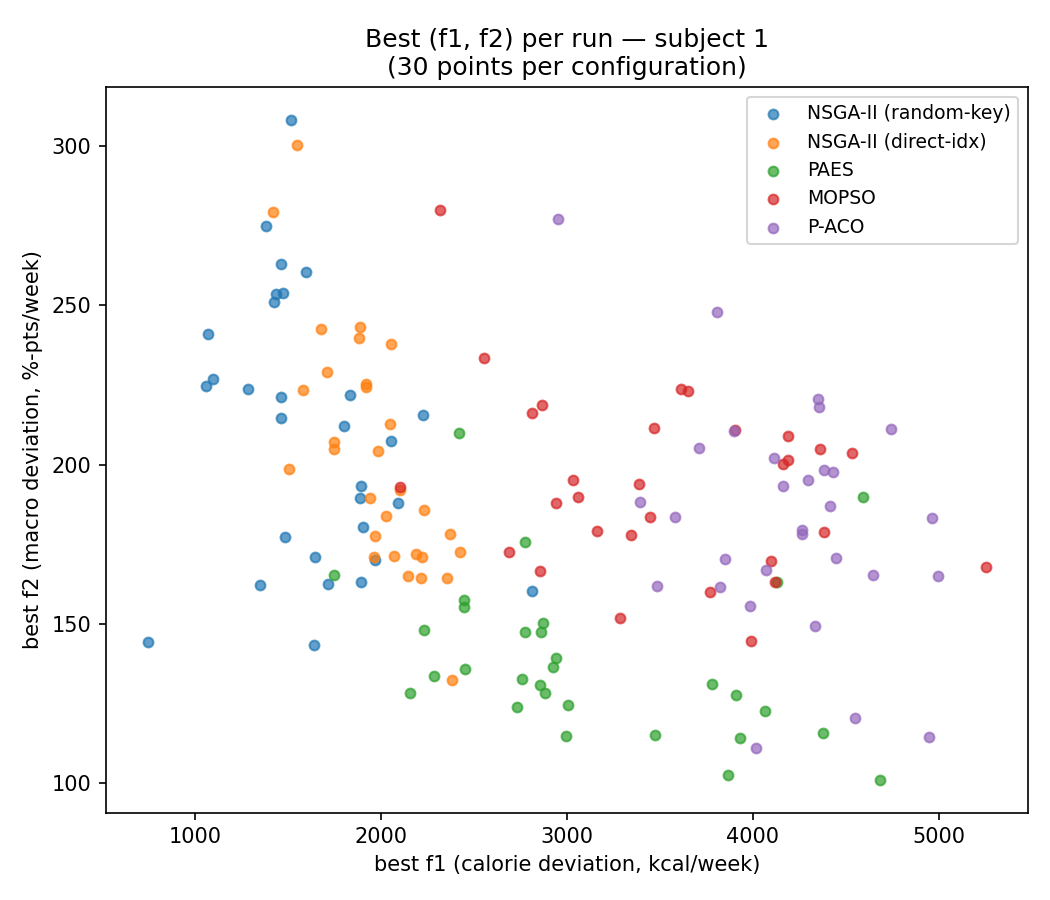
\includegraphics[width=0.7\textwidth]{experiments/best_pts_subject_1.png}
\caption{Cloud of best $(f_1, f_2)$ values per run for subject 1, coloured by configuration. NSGA-II variants concentrate in the bottom-left (best on both objectives); PAES and MOPSO populate intermediate regions; the scalarised PSO collapses to a single point per run.}
\label{fig:bestpts}
\end{figure}

\subsection{Discussion}

\paragraph{NSGA-II is the dominant algorithm family.} All four NSGA-II configurations occupy the top four ranks on both hypervolume and IGD. The closest non-NSGA-II competitor (MOPSO) is significantly worse on hypervolume ($p_{\mathrm{adj}}\!<\!10^{-13}$ in Wilcoxon+Shaffer). The hyperparameter sweep confirms this from a different angle: in isolation, NSGA-II at \texttt{pop=80, mut=0.1} reaches HV $\approx$ 1.34 million, well above the best PAES (706k), best MOPSO (974k) and best scalarised PSO (5k) settings on the same subject.

\paragraph{Random-key matches direct-index quality but is $2.4\times$ faster.} The hypervolume difference between \texttt{nsga2\_di\_repair} and \texttt{nsga2\_rk\_repair} is statistically negligible ($p_{\mathrm{adj}}\!=\!0.82$ in the Wilcoxon+Shaffer test), but the IGD ranking favours the random-key variant and the runtime gap is large (8.9~s vs.\ 21.6~s). The runtime advantage stems from the random-key repair being a trivial $O(n)$ clamp into $[0, 1]$ that does not require re-evaluating the fitness function, whereas the direct-index repair re-runs fitness whenever a gene is replaced.

\paragraph{Constraint handlers are equivalent in our setup.} The three direct-index configurations (\texttt{repair}, \texttt{penalty}, \texttt{death\_penalty}) produce identical hypervolume, IGD, spacing, $f_1$ and $f_2$, with $p_{\mathrm{adj}}\!=\!1.0$ in the Wilcoxon+Shaffer pairwise test. The reason is structural rather than statistical: our domain-aware mutation always picks each gene from $D_j$, so no infeasible candidate is ever produced and no handler is ever triggered. The only observable difference between the three handlers is runtime --- \texttt{repair} is the slowest because of its always-on fitness re-evaluation, \texttt{penalty} is the fastest because it only counts violations. To meaningfully differentiate the three techniques one would need an unrestricted variator that can produce infeasible candidates, which we identify as the most promising future-work item.

\paragraph{PAES has the best per-point macronutrient quality but the weakest Pareto coverage.} The mean best $f_2$ for PAES is $129.0$, the lowest of the seven configurations. Hypervolume, however, is roughly 40\% of NSGA-II's. This is the expected trade-off for a $(1{+}1)$-ES with grid archiving: it exploits one trajectory deeply but does not actively diversify the front. The hyperparameter sweep additionally shows that PAES is insensitive to the archive size in this problem because the archive never fills up.

\paragraph{Scalarised PSO is a baseline reference, not a competitor.} It collapses to a single point per run, which gives it a Pareto front of size 1, near-zero hypervolume and the worst IGD. It does win on runtime, but for a multi-objective deliverable that is not a useful trade-off.

\subsection{Code repository}

The full source code, tests and experiment notebook required to reproduce every figure and table in this section is hosted at:

\begin{center}
\url{https://github.com/gjorgiandonovski/Multi-objective-Diet-Optimization-Problem}
\end{center}

%==============================================
% CONCLUSION
%==============================================
\section{Conclusion and future work}

This project addressed the multi-objective diet optimisation problem with two evolutionary algorithms (NSGA-II, PAES), two swarm intelligence algorithms (a scalarised PSO baseline and a Pareto-based MOPSO), two encodings (direct-index, random-key) and three constraint handlers (repair, penalty, death penalty). Across 1{,}050 statistically validated runs on five real user profiles and 2{,}616 foods --- complemented by a within-algorithm hyperparameter sensitivity sweep on the demo subject --- the recommended configuration is \textbf{NSGA-II with the random-key encoding, the repair handler, mutation rate $0.1$ and population size $80$}. It is statistically tied with NSGA-II direct-index on hypervolume, achieves the lowest IGD overall and is $2.4\times$ faster than its direct-index counterpart. PAES yields the best per-point macronutrient adjustment but at the cost of significantly weaker Pareto coverage; MOPSO is markedly better than scalarised PSO on every multi-objective indicator while remaining computationally cheap; and the scalarised PSO baseline serves as a clear lower-bound reference rather than as a competitor.

A side finding that turned out to be educationally relevant is that the three constraint handlers became indistinguishable in our setup: because mutation always picks genes from valid domains, no infeasible candidate is ever produced and the handlers never fire. We treat this as a documented limitation and as motivation for the most natural follow-up work.

\paragraph{Suggested future directions.}
\begin{enumerate}[leftmargin=1.4em, itemsep=0.1em]
\item Replace the domain-aware variator with a naive (unrestricted) one so that the three constraint handlers can be properly differentiated.
\item Add Ant Colony Optimisation (course topic 3.2) as a third swarm method; the constructive nature of ACO makes it a natural fit for slot-by-slot meal-plan construction.
\item Implement a memetic NSGA-II variant (course topic 7.1) by injecting a one-step local search after each generation.
\item Parallelise the per-replicate evaluation loop to bring the wall-clock cost of the main grid below 30 minutes.
\item Extend the fitness function to incorporate the user-profile preferences, dislikes and allergies that the database carries but the present formulation ignores.
\end{enumerate}

%==============================================
% REFERENCES
%==============================================
\section*{References}

\begin{enumerate}[leftmargin=1.6em]
\item Deb, K., Pratap, A., Agarwal, S., \& Meyarivan, T. (2002). \textit{A fast and elitist multiobjective genetic algorithm: NSGA-II}. IEEE Transactions on Evolutionary Computation, 6(2), 182-197.
\item Knowles, J., \& Corne, D. (2000). \textit{Approximating the nondominated front using the Pareto archived evolution strategy}. Evolutionary Computation, 8(2), 149-172.
\item Coello, C. A. C., Pulido, G. T., \& Lechuga, M. S. (2004). \textit{Handling multiple objectives with particle swarm optimization}. IEEE Transactions on Evolutionary Computation, 8(3), 256-279.
\item Nebro, A. J., Durillo, J. J., Garcia-Nieto, J., Coello Coello, C. A., Luna, F., \& Alba, E. (2009). \textit{SMPSO: A new PSO-based metaheuristic for multi-objective optimization}. IEEE Symposium on Computational Intelligence in Multi-Criteria Decision-Making, 66-73.
\item Kennedy, J., \& Eberhart, R. (1995). \textit{Particle swarm optimization}. Proceedings of ICNN'95, vol.\ IV, 1942-1948.
\item Schott, J. R. (1995). \textit{Fault tolerant design using single and multicriteria genetic algorithm optimization}. Master's thesis, Massachusetts Institute of Technology.
\item Zitzler, E., \& Thiele, L. (1999). \textit{Multiobjective evolutionary algorithms: A comparative case study and the strength Pareto approach}. IEEE Transactions on Evolutionary Computation, 3(4), 257-271.
\item Friedman, M. (1937). \textit{The use of ranks to avoid the assumption of normality implicit in the analysis of variance}. Journal of the American Statistical Association, 32(200), 675-701.
\item Wilcoxon, F. (1945). \textit{Individual comparisons by ranking methods}. Biometrics Bulletin, 1(6), 80-83. (Mann \& Whitney, 1947, extended this idea to independent samples; we use the original paired form.)
\item Holm, S. (1979). \textit{A simple sequentially rejective multiple test procedure}. Scandinavian Journal of Statistics, 6(2), 65-70.
\item Shaffer, J. P. (1986). \textit{Modified sequentially rejective multiple test procedures}. Journal of the American Statistical Association, 81(395), 826-831.
\item Garrett, A. (2012). \textit{Inspyred: Bio-inspired algorithms in Python}. \url{https://aarongarrett.github.io/inspyred/}
\item Quesada Pajares, J. (2024). \textit{NutritionPlanning: food database and reference scripts for the BAO course}. \url{https://github.com/javierquesadapajares/NutritionPlanning}
\item Coello, C. A. C., Lamont, G. B., \& Van Veldhuizen, D. A. (2007). \textit{Evolutionary Algorithms for Solving Multi-Objective Problems} (2nd ed.). Springer.
\end{enumerate}

\end{document}
